% !TEX root = ./rapport.tex

% ─────────────────────────────────────────────────────────────
% Plan des annexes
% ─────────────────────────────────────────────────────────────
\chapter*{Plan des annexes}
\addcontentsline{toc}{chapter}{Plan des annexes}
\markboth{Plan des annexes}{}

\begin{description}[leftmargin=3.5cm, style=sameline, font=\normalfont\bfseries]
  \item[Annexe I]   Formulaire de création d'un employé~: données personnelles, département et poste
  \item[Annexe II]  Tableau de bord employé~: suivi des demandes et indicateurs de statut
  \item[Annexe III] Interface d'entretiens~: planification et décisions
  \item[Annexe IV]  Vue de prédiction d'attrition~: KPI globaux et liste des employés par score de risque
  \item[Annexe V]   Matrice RBAC de Synapse
\end{description}

\cleardoublepage

\captionsetup{font=footnotesize}

% ─────────────────────────────────────────────────────────────
\chapter{Formulaire de création d'un employé}
\label{ann:create_emp}
% ─────────────────────────────────────────────────────────────
\vspace*{-0.8cm}
\begin{figure}[H]
  \centering
  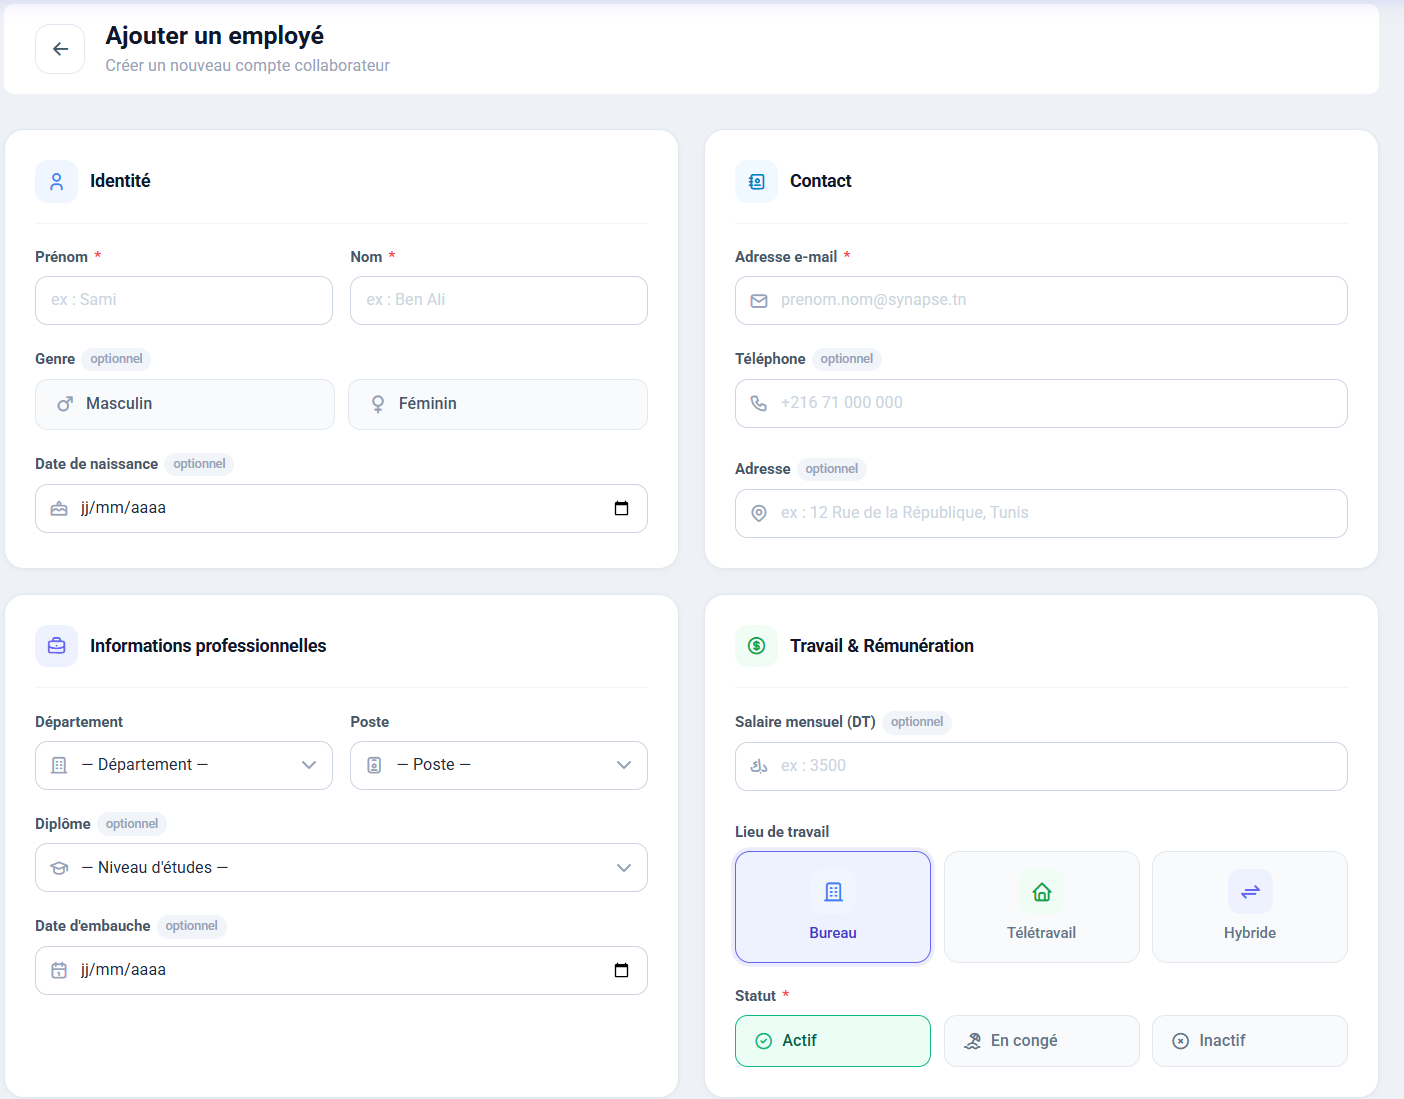
\includegraphics[width=0.60\textwidth,keepaspectratio]{images/screenshot_create_employee.png}
  \caption{Formulaire de création d'un employé~: données personnelles, département et poste}
  \label{fig:create_emp_form}
\end{figure}

% Annexe II sur la même page — on neutralise le \clearpage interne de \chapter
{
  \let\clearpage\relax
  \let\cleardoublepage\relax
% ─────────────────────────────────────────────────────────────
\chapter{Tableau de bord employé~: suivi des demandes}
\label{ann:mes_demandes}
% ─────────────────────────────────────────────────────────────
}

\begin{figure}[H]
  \centering
  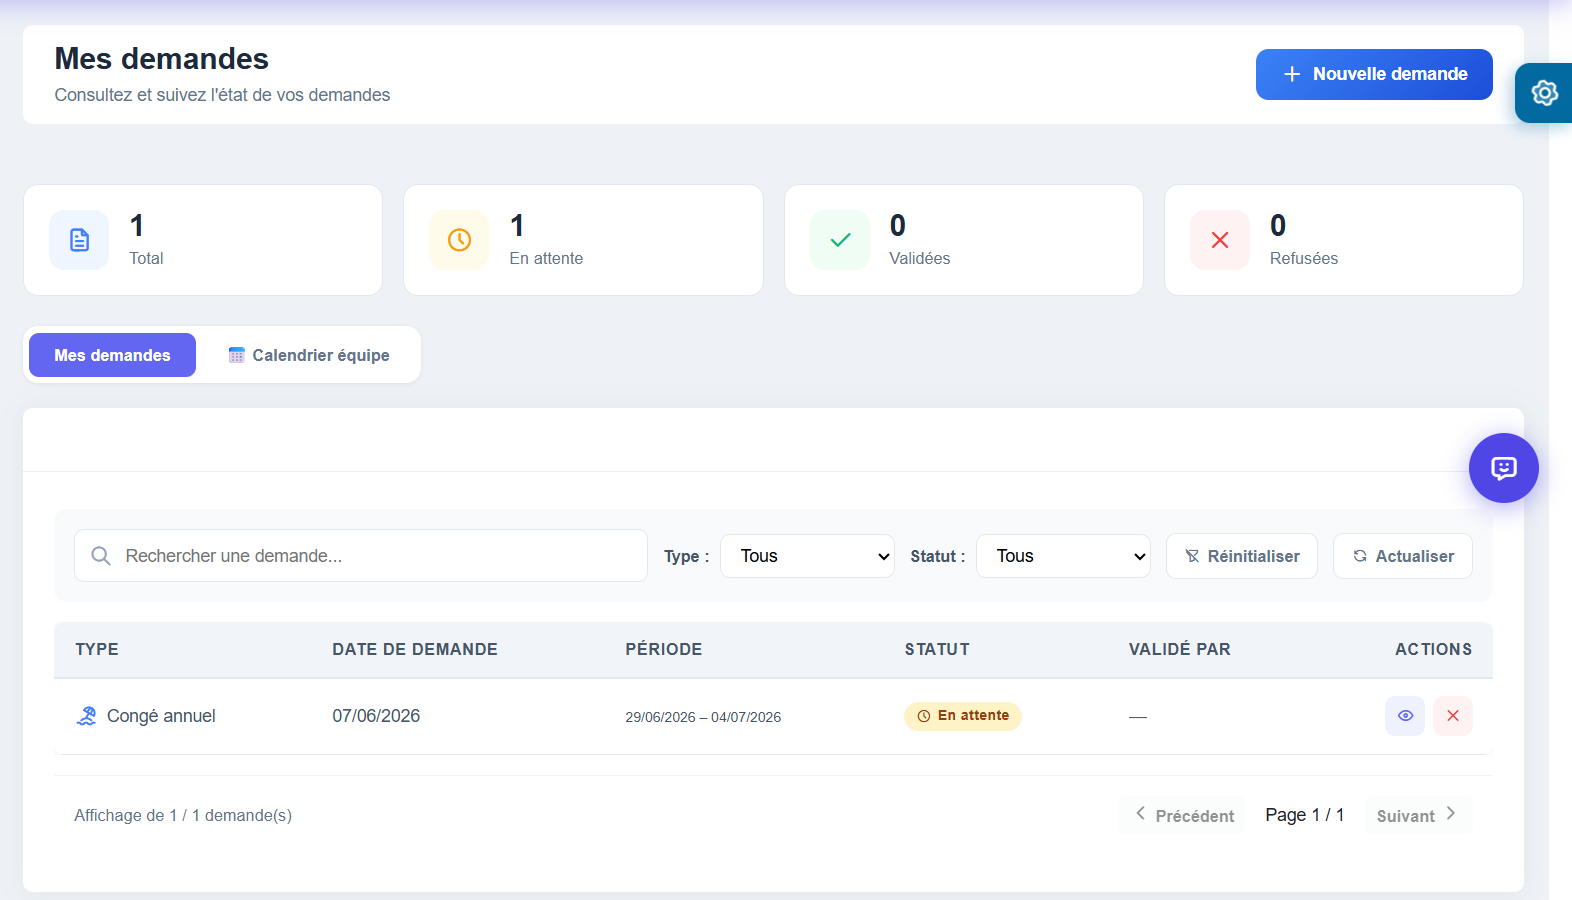
\includegraphics[width=0.70\textwidth,keepaspectratio]{images/screenshot_mes_demandes.png}
  \caption{Tableau de bord employé~: suivi des demandes et indicateurs de statut}
  \label{fig:mes_demandes}
\end{figure}

\cleardoublepage

% ─────────────────────────────────────────────────────────────
\chapter{Interface d'entretiens~: planification}
\label{ann:interviews}
% ─────────────────────────────────────────────────────────────

\begin{figure}[H]
  \centering
  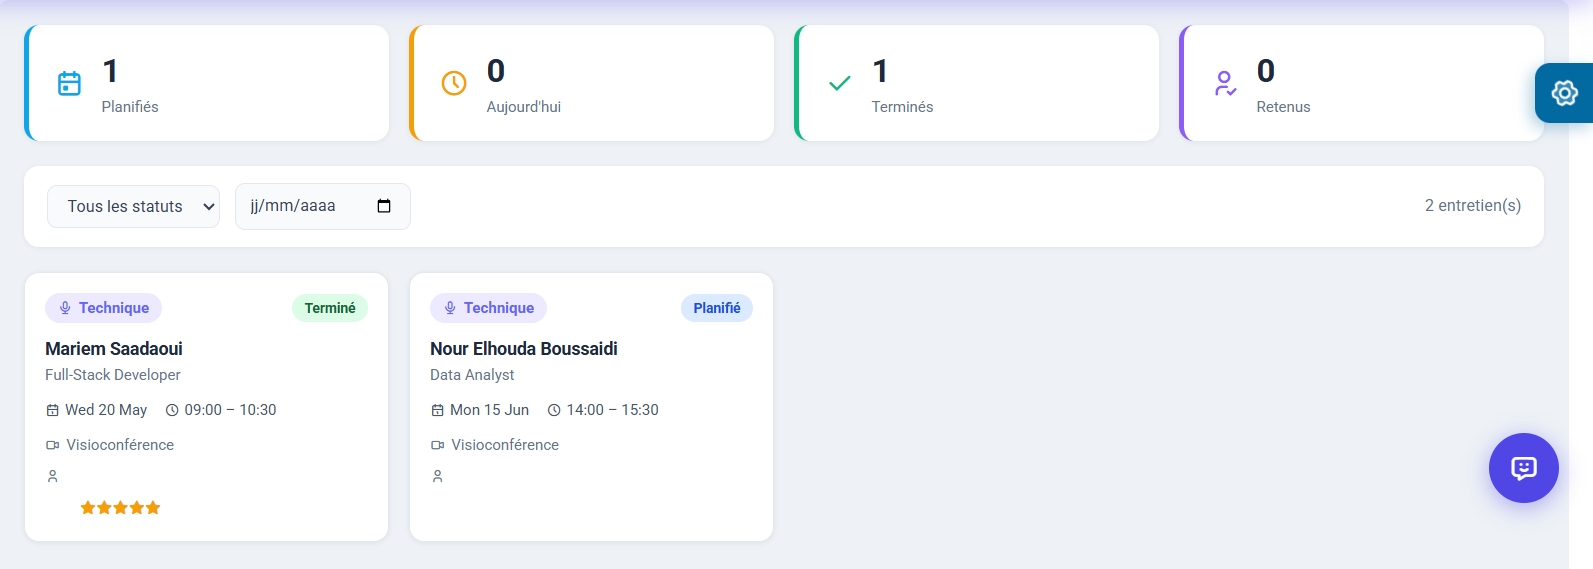
\includegraphics[width=0.70\textwidth,keepaspectratio]{images/screenshot_interviews.png}
  \caption{Interface d'entretiens~: planification}
  \label{fig:interviews_view}
\end{figure}

% Annexe IV sur la même page — on neutralise le \clearpage interne de \chapter
{
  \let\clearpage\relax
  \let\cleardoublepage\relax
% ─────────────────────────────────────────────────────────────
\chapter{Vue de prédiction d'attrition}
\label{ann:attrition}
% ─────────────────────────────────────────────────────────────
}

\begin{figure}[H]
  \centering
  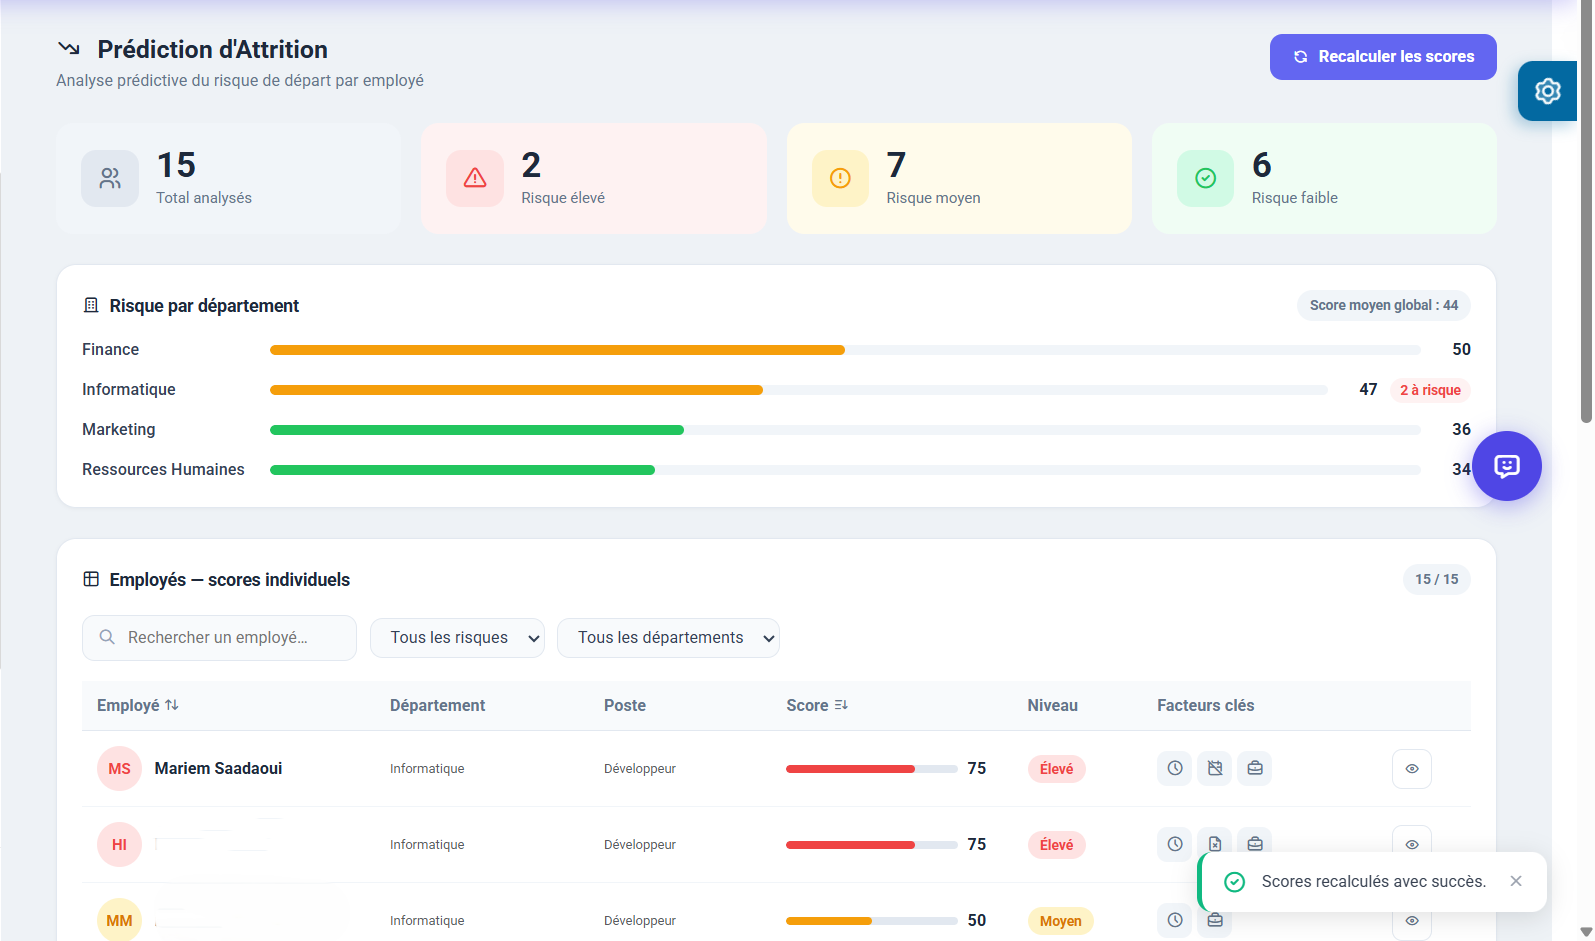
\includegraphics[width=0.70\textwidth,keepaspectratio]{images/screenshot_attrition_main.png}
  \caption{Vue de prédiction d'attrition~: KPI globaux et liste des employés par score de risque}
  \label{fig:attrition_main}
\end{figure}

\cleardoublepage

% ─────────────────────────────────────────────────────────────
\chapter{Matrice RBAC de Synapse}
\label{ann:rbac}
% ─────────────────────────────────────────────────────────────

\begin{table}[H]
\centering
\caption{Matrice RBAC de Synapse}
\label{tab:rbac_matrix}
\footnotesize\renewcommand{\arraystretch}{0.85}
\begin{tabularx}{\textwidth}{VLVCVCVCVCVCVCV}
\rowcolor{headerblue!55}
\hline
\textbf{Fonctionnalité} & \textbf{EMPLOYE} & \textbf{CHEF} & \textbf{RH} & \textbf{ADMIN\_RH} & \textbf{DG} & \textbf{COMITE} \\
\hline
Déposer une demande RH & \faCheckCircle & \faCheckCircle & \faCheckCircle & \faCheckCircle & & \\
\hline
Valider (niveau Chef) & & \faCheckCircle & & \faCheckCircle & & \\
\hline
Valider (niveau RH) & & & \faCheckCircle & \faCheckCircle & & \\
\hline
Créer/modifier un employé & & & & \faCheckCircle & & \\
\hline
Approuver un prêt (DG) & & & & & \faCheckCircle & \\
\hline
Voter (comité crédit) & & & & & & \faCheckCircle \\
\hline
Générer des rapports PDF & & \faCheckCircle & \faCheckCircle & \faCheckCircle & & \\
\hline
Consulter l'attrition & & & \faCheckCircle & \faCheckCircle & & \\
\hline
Chat interne & \faCheckCircle & \faCheckCircle & \faCheckCircle & \faCheckCircle & & \\
\hline
Gérer les projets/tâches & & \faCheckCircle & & \faCheckCircle & & \\
\hline
Consulter ses propres tâches & \faCheckCircle & \faCheckCircle & \faCheckCircle & \faCheckCircle & & \\
\hline
\end{tabularx}
\end{table}
